\section{Hindernisse in der Simulation}
\label{sec:implementation_boundaries}

Bisher wurde das Hindernisfeld \PimiddyInlineCode{boundary} als
gegeben angenommen. Nun sollen Möglichkeiten vorgestellt werden, das
Feld mit Hinderniswerten zu füllen. Es wird zuerst ein Ansatz
beschrieben, bei dem Hindernisse aus primitiven Formen zusammengesetzt
werden. Danach werden Verfahren vorgestellt, um direkt aus einer
Meshdatei ein Hindernisfeld zu erzeugen.

\subsection{Einfacher Ansatz}

Oft ist die Geometrie von Hindernissen relativ einfach gestaltet, oder
sie wird speziell für die Simulation vereinfacht. Das angezeigte Mesh
hat dann gegebenenfalls wesentlich mehr Details als das diskretisierte
Hindernisfeld. Bewegen sich die Partikel schnell genug \Pimiddybzw
löscht man die Partikel erst eine gewisse Zeit nach der Kollision mit
den Hindernissen, ist der Detailunterschied nicht zu merken.

Es bietet sich daher an, die Hindernisse aus einfachen geometrischen
Formen wie Kugeln oder Quadern zusammenzusetzen. Diese Formen lassen
sich sehr einfach diskretisieren, was im folgenden besprochen werden soll.

Gegeben einer Menge von geometrischen Formen und einem Anfangs mit $0$
gefüllten Hindernisfeld, kann das endgültige Hindernisfeld
inkrementell konstruiert werden, indem immer weiter einzelne
Hindernisse hinzugefügt werden (sprich, Werte auf $1$ gesetzt
werden). Für jedes Primitiv benötigt man einen Kernel, der die
geometrischen Eigenschaften (\PimiddyzB{} Ausdehnung) sowie
\PimiddyInlineCode{boundary} erhält.

Für einen Quader $Q$, gegeben durch die drei Intervalle
$[x_1,x_2],[y_1,y_2],[z_1,z_2]$, ist dieser Kernel sehr einfach
gestaltet. Für jeden Voxel muss er testen, ob dessen Position
innerhalb des Quaders ist.

Für eine Kugel, gegeben durch einen Radius $r$ und eine Position
$(x,y,z)$ muss für jeden Voxel mit Position $(v_x,v_y,v_z)$ die
Kugelungleichung ausgewertet werden:

\begin{align}
{(x-v_x)}^2 + {(y-v_y)}^2 + {(z-v_z)}^2 \leq r^2
\end{align}

Ist sie wahr, wird der Voxel auf 1 gesetzt. Ähnlich einfach lässt sich
ein Ellipsoid behandeln, welcher durch drei Radien $r_x,r_y,r_z$ und eine
Position $(x,y,z)$ gegeben ist. Seine Ungleichung lautet:

\begin{align}
\frac{{(x-v_x)}^2}{r_x} + \frac{{(y-v_y)}^2}{r_y} + \frac{{(z-v_z)}^2}{r_z} \leq 1
\end{align}

Diese Art, Hindernisse einzubringen, ist allerdings sehr
zeitaufwändig, da stets zwei Modelle zu erstellen sind --- eins zur
Anzeige, bestehend aus einer Menge von Dreiecken, und eins für die
Simulation, bestehend aus geometrischen Formen. Die Konvertierung dieser
Formen zu Dreiecksnetzen ist zwar ohne Probleme möglich, es ist jedoch
ein sehr unnatürlicher Arbeitsablauf und es existieren keine Tools,
die dies vereinfachen könnten.

\subsection{Komplexe Hindernisse}

Es wäre günstiger, aus dem Mesh, was später angezeigt wird, das
Hindernisfeld zu gewinnen --- oder notfalls aus einem leicht
vereinfachten Mesh, welches rein visuell interessante Objekte nicht
enthält. Diesen Vorgang nennt man \PimiddyBegriff{Voxelization}. Im
Weiteren wird ein simpler Algorithmus vorgeschlagen, um diese Aufgabe
zu lösen. Für größere Felder ist dieser Algorithmus allerdings
ungeeignet, daher werden Alternativen besprochen.
\begin{figure}[h]
\centering
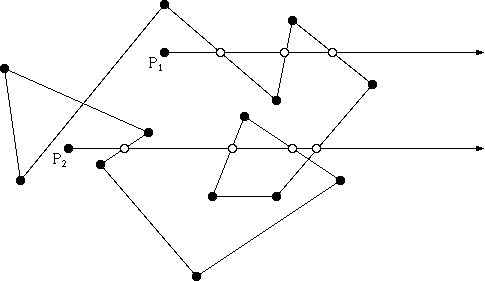
\includegraphics[width=10cm]{images/point_in_polygon}
\caption{Der einfache Test, ob ein Punkt in einem Körper enthalten ist, hier in zwei Dimensionen. $P_1$ hat 3 Schnittpunkte und ist innerhalb, $P_2$ hat 4 und ist somit außerhalb.}
\label{fig:implementation_boundaries_point_in_polygon}
\end{figure}
Gegeben sei eine Menge von Dreiecken, gegeben durch ihre Eckpunkte
(weitere Eigenschaften wie Normalen und Texturkoordinaten sind für die
Umwandlung nicht interessant). Die Menge von Dreiecken soll einen
geschlossenen Körper bilden, Löcher oder Überschneidungen sind nicht
erlaubt. Unter diesen Voraussetzungen lässt ich für jeden Gitterpunkt
in \PimiddyInlineCode{boundary} entscheiden, ob dieser innerhalb des
Körpers ist oder außerhalb: Man betrachtet eine Halbgerade vom
Gitterpunkt aus und zählt die Schnittpunkte der Geraden mit allen
Dreiecken des Körpers. Bei einer geraden Anzahl von Schnittpunkten ist
der Punkt außerhalb, sonst innerhalb (siehe
\cref{fig:implementation_boundaries_point_in_polygon}).

Der Test ist arithmetisch sehr einfach gestaltet und
performant. Allerdings ist seine Laufzeit immernoch $O(n^3 \cdot k)$,
wobei $n$ die Größe des Gitters angibt und $k$ die Anzahl an
Dreiecken. Bei einem $64^3$ großen Feld und einem hinreichend
komplexen Modell mit $3.000$ Dreiecken kommt man bereits auf
786.432.000 Tests.

Die Implementierung eines effizienteren Verfahrens übersteigt den
Rahmen dieser Arbeit allerdings deutlich, daher wurde auf das Tool
\emph{binvox} zurückgegriffen (\cite{binvox2012}). Es verwendet den
Algorithmus aus \cite{Nooruddin2003}, der auf \PimiddyQuotes{Ray
Stabbing} basiert, einer Abwandlung des eben beschriebenen
Verfahrens. Das Tool arbeitet parallel auf der GPU und liefert in
Sekunden Ergebnisse. Als Eingabe erhält es die Modeldatei im
obj-Dateiformat, welche vom Programm auch direkt zur Anzeige verwendet
wird. Die Ausgabe erfolgt in einem eigens geschrieben Dateiformat, dem
binvox-Format\cite{binvoxfileformat2012}. Eine
\PimiddyInlineCode{.binvox}-Datei hat den folgenden, einfachen Aufbau:

\begin{minted}{java}
#binvox 1
dim 128 128 128
translate -0.120158 -0.481158 -0.863158
scale 7.24632
data
...
\end{minted}

Die erste Zeile gibt die Version des Dateiformats an. Zum jetzigen
Zeitpunkt gibt es nur Version 1. Die nächste Zeile gibt die
Dimensionen des Gitters an. Die Werte für
\PimiddyInlineCode{translate} und \PimiddyInlineCode{scale} geben an,
wie das Gitter verschoben und skaliert werden muss, um mit dem
vorgegebene Model übereinzustimmen.

Danach folgen die eigentlichen Daten als rohe Bytes. Um Platz bei
großen Gittern zu sparen, sind sie \emph{lauflängenkodiert}. Das
Datensegment enthält eine Folge von Byte-Paaren. Das erste Byte in
einem Paar gibt an, ob eine Folge von Nullen oder Einsen folgt. Das
zweite Byte gibt an, wie viele Nullen oder Einsen folgen.

Die lineare Folge von Gitterpunkten wird mit der Festlegung zum
dreidimensionalen Gitter, dass sich die $y$-Koordinate am schnellsten
verändert, dann die $x$-Koordinate, dann die $z$-Koordinate.

\begin{figure}
	\begin{subfigure}[t]{0.5\textwidth}
		\centering
		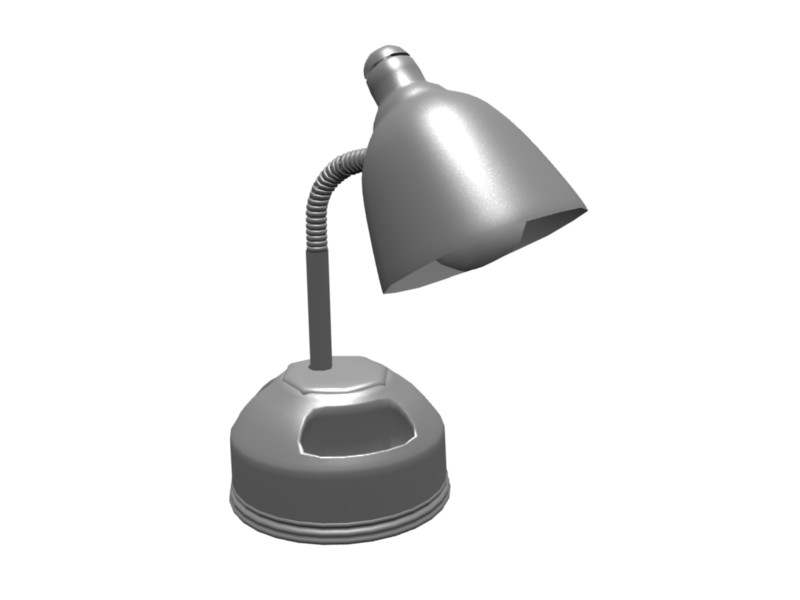
\includegraphics[width=\textwidth]{images/lamp_obj}
		\caption{Das Modell einer Lampe}
	\end{subfigure}
    ~
	\begin{subfigure}[t]{0.5\textwidth}
		\centering
		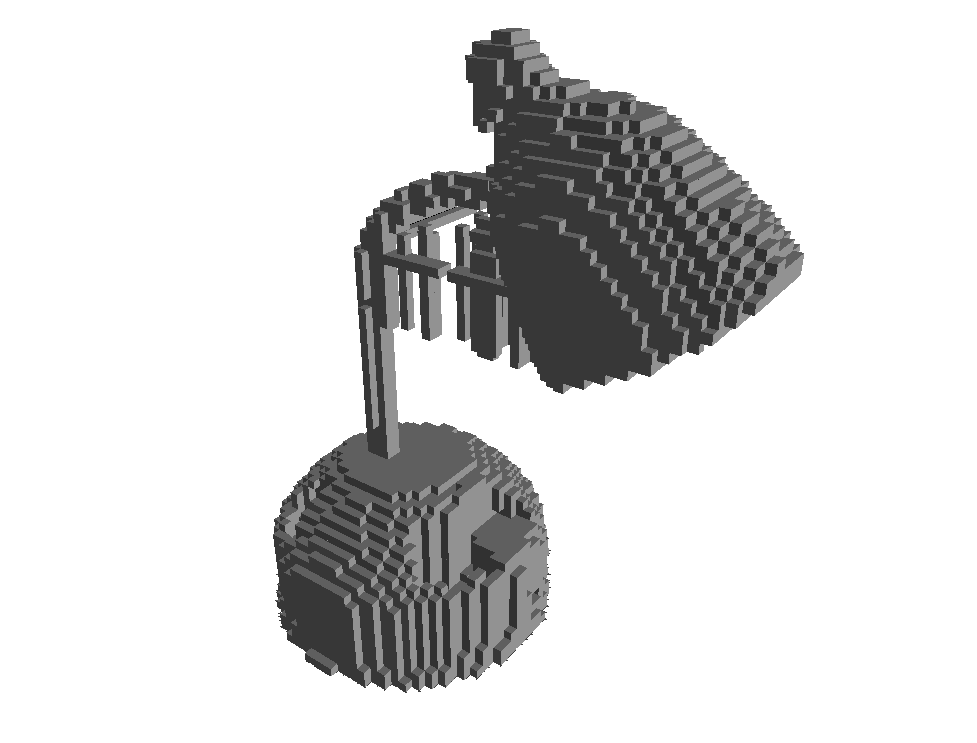
\includegraphics[width=\textwidth]{images/lamp_discrete}
		\caption{Die von binvox diskretisierte Version der Lampe}
	\end{subfigure}
	\caption{Das Tool binvox bei der Arbeit.}
\end{figure}